\documentclass{llncs}
\usepackage{times}
\usepackage{graphicx}
\usepackage{latexsym}
\usepackage{multirow}
% \usepackage[scaled=.8]{beramono}
\usepackage[usenames,dvipsnames,svgnames,table]{xcolor}
\definecolor{light-gray}{gray}{0.95}
\usepackage[fleqn]{amsmath}
\usepackage{microtype}
\usepackage{verbatim}
\usepackage{paralist}
\usepackage{url}
\usepackage{listings}
\lstset{ %
   language=prolog,
%  frame=l,                     % adds a frame around the code
%   basicstyle=\footnotesize,  % use courier
   basicstyle=\footnotesize\ttfamily,	% use courier
   breaklines=true,
   xleftmargin=0.5em,
   xrightmargin=-0.5em,
   aboveskip=0.5em,
   belowskip=0.5em,
%  belowcaptionskip=5em,
   numbers=left,
   backgroundcolor=\color{light-gray},
   frame=single,
   framerule=0pt
}
\usepackage[usenames,dvipsnames]{xcolor}
\usepackage{todonotes}
\def\mnote#1{\todo[color=Goldenrod,size=\scriptsize]{Matt: #1}}
\def\jnote#1{\todo[color=CornflowerBlue,size=\scriptsize]{Julian: #1}}
\def\snote#1{\todo[color=WildStrawberry,size=\scriptsize]{Steve: #1}}

\setlength{\jot}{0pt}


\begin{document}

% Long paper page limit: 12 pages

\title{Describing Possible Narrative Worlds with Interval Temporal Logic and Kripke Models}


\author{Matt Thompson\inst{1,}\inst{2} \and Steve Battle\inst{2} \and Julian Padget\inst{1} }
\institute{Department of Computer Science,\\
University of Bath, UK\\
\email{\{m.r.thompson,j.a.padget\}@bath.ac.uk}
\and
The University of the West of England (UWE), UK\\
\email{steve.battle@uwe.ac.uk}}

\maketitle
\bibliographystyle{plain}


\begin{abstract}
  Abstract goes here.
\end{abstract}

\section{Introduction}
\mnote{Clarify what the message is/what's desirable. What are the shortcomings of current approaches, how do we solve them?}
Agent-based approaches to narrative generation must strike a balance between authorial control (writing a story structure), and agent's actions (allowing characters to fill in the details of a story). One way to overcome this is to allow the author to describe the structure of a story in a way which constrains the available actions of the agents.

This introduces a problem: if there are multiple paths through a narrative (chosen by user interaction), how can an author describe alternative scenarios without explicitly writing out every single branch of the story?

A wide variety of approaches have been taken to address this issue. A popular and effective one is to combine the use of a \emph{drama manager} with a Multi Agent System in order to regulate the actions of intelligent agents playing the parts of characters, telling them which actions to take in order to conform to a story. One of the first implementations of this approach was the Oz project at Carnegie Mellon University \cite{bates1992virtual}, ideas from which were later developed to become Mateas and Stern's \emph{Fa{c}cade} \cite{mateas2003faccade}.

\mnote{Goal is to support greater agency for actors}
An approach that we have explored is to model the narrative as an institution of social norms, describing what the character agents are \emph{permitted} and \emph{obliged} to do at certain points in the story \cite{thompson-et-al:2015}. The advantage of this approach is that it merely suggests permitted actions to the agents, which have some degree of control over the actions they finally choose to carry out. For example, in an interactive narrative, a player could push a character so far that it causes them to deviate from the normal course of the story (albeit at some cost to the character agent).

Other approaches to balancing authorial control with player or character agency include the use of director agents \cite{lee2011learning}, reincorporation of player actions back into the narrative \cite{tomaszewski2011use} and mediation to prevent narrative-breaking actions \cite{robertson2013modelling}.

\mnote{Need to include all the work done with planners (Riedl, Young, etc) here}

In this paper we describe the use of modal logic, Interval Temporal Logic \cite{della2013interval}, and Kripke models \cite{kripke1963semantical} to describe the many paths which a narrative can take.

This approach is influenced by Marie-Laure Ryan's work describing possible worlds \cite{ryan1991possible} in the field of narratology. Ryan describes how, in the field of interactive narrative, the path one takes through a story is but one realisation of many possible story worlds. She asserts the link between possible worlds and modal logic, and Saul Kripke's work in particular. Taking this as inspiration, we formally develop these ideas in this paper.

We begin with a description of the narrative formalism we use for our approach, Propp's Morphology of the Folktale \cite{propp1968morphology}, in section \ref{sec:propp}. The use of this formalism is demonstrated with an example from the \emph{Punch and Judy} story world in section \ref{sec:pjexample}. Section \ref{sec:propplogic} implements this example using Interval Temporal Logic and modal logic. Following this, Kripke models are then implemented using the LoTREC tableaux prover \cite{del2001lotrec} (section \ref{sec:kripke})./mnote{Why do you want to use ITL \& Kripke models? What does this allow us to do?}
\mnote{Add relevance to digital storytelling. Logic allows richer capture of story structure}

\section{Propp's Morphology of the Folktale}\label{sec:propp}
To express story events in modal logic, we need some sort of formalisation for the analysis of the story~-- rather than an arbitrary selection of features~-- and so we look to narrative theory for inspiration. Instead of describing parts of the Punch and Judy story explicitly (such as `Punch is expected to hit the policeman in this scene'), it is desirable to describe scenes in a more abstract way using roles (`The villain fights the victim in this scene'). The use of more general story fragments allows us to reuse them in multiple scenes, or even in other stories.

Narratology, and structuralism in particular, supply such generalised building blocks for stories. Russian formalism is an early movement in narrative theory that sought to formalise the elements of narrative, and Vladimir Propp was a prominent figure in this school.  One outcome of this movement was Propp's 1928 formalism derived from the study of Russian folktales, \emph{The Morphology of the Folktale} \cite{propp1968morphology}, which is what we use to build a model to direct the course of the narrative.  In this formalism, Propp identifies recurring characters, which become roles, and motifs, which become action fragments, in Russian folklore, distilling them down to a concise syntax with which to describe stories. Propp's functional, event-driven style translates comfortably to an institution comprised of event-based norms. However, while these action fragments fit the Punch and Judy story adequately, we note that the role labels can sound rather awkward because of the apparent semantic import of the textual label.

In Propp's formalism, characters have \emph{roles}, such as \emph{hero}, \emph{villain}, \emph{dispatcher}, \emph{false hero}, and more. Characters performing a certain role are able to perform a subset of \emph{story moves}, which are actions that make the narrative progress. For example, the \emph{dispatcher} might send the \emph{hero} on a quest, or the \emph{victim} may issue an \emph{interdiction} to the \emph{villain}, which is then \emph{violated}.

Propp defines a total of 31 distinct story functions. Each function is given a number and symbol in order to create a succinct way of describing entire stories. Examples of such functions are:

\begin{compactitem}
  \item One of the members of a family absents himself from home: \emph{absentation}.
  \item An interdiction is addressed to the hero: \emph{interdiction}.
  \item The victim submits to deception and thereby unwittingly helps his enemy: \emph{complicity}.
  \item The villain causes harm or injury to a member of the family: \emph{villainy}.
\end{compactitem}

Each of these functions can vary in subtle ways. For example, the \emph{villainy} function can be realised as one of 19 distinct forms of villainous deed, including \emph{the villain abducts a person}, \emph{the villain seizes the daylight}, and \emph{the villain makes a threat of cannibalism}.
These functions are enacted by characters following certain roles. Each role (or \emph{dramatis persona} in Propp's definition) has a \emph{sphere of action} consisting of the functions that they are able to perform at any point in the story. Propp defines seven roles each of which has distinct spheres of action: \emph{villain}, \emph{donor}, \emph{helper}, \emph{princess}, \emph{dispatcher}, \emph{hero}, and \emph{false hero}.
In a typical story, one story function will follow another as the tale progresses in a sequential series of cause and effect. However, Propp's formalism does also allow for simultaneous story functions.

\subsection{Propp Example: Sausages and Crocodile Scene}\label{sec:pjexample}
To provide some context for Punch and Judy, since it is a peculiarly British phenomenon, although with Italian origins, we quote from Wikipedia:
\begin{quote}\small
Punch and Judy is a traditional, popular, and usually very violent puppet show featuring Mr Punch and his wife, Judy. The performance consists of a sequence of short scenes, each depicting an interaction between two characters, most typically Mr Punch and one other character (who usually falls victim to Mr. Punch's club). It is often associated with traditional British seaside culture.
The Punch and Judy show has roots in the 16th-century Italian commedia dell'arte. \\
\hfill{\footnotesize
\url{http://en.wikipedia.org/wiki/Punch_and_Judy}, retrieved 2015-05-06.}
\end{quote}

The common elements of Punch and Judy are easily described in terms of Propp's story functions. Here we pick one scene to use as an example: the scene where Punch battles a crocodile in order to safeguard some sausages.  In this scene, Joey the clown (our narrator) asks Punch to guard the sausages. Once Joey has left the stage, a crocodile appears and eats the sausages. Punch fights with the crocodile, but it escapes. Joey then returns to find that his sausages are gone.
The corresponding story functions are:
\begin{enumerate}
  \item Joey tells Punch to look after the sausages (\emph{interdiction}).
  \item Joey has some reservations, but decides to trust Punch (\emph{complicity}).
  \item Joey gives the sausages to Punch (\emph{provision or receipt of a magical agent}).
  \item Joey leaves the stage (\emph{absentation}).
  \item A crocodile enters the stage and eats the sausages (\emph{violation}).
  \item Punch fights with the crocodile (\emph{struggle}).
  \item Joey returns to find that the sausages are gone (\emph{return}).
\end{enumerate}

Some story functions map to Punch and Judy better than others (for example, it is debatable as to whether or not the sausages can be considered a ``magical agent''), but Propp's formalism seems well suited to Punch and Judy for the most part. The advantage of using Propp for the Punch and Judy story domain is that the story function concept maps well to the idea of internal events in institutional models.

\section{Combining Interval Temporal Logic and Modal Logic for Propp}\label{sec:propplogic}
\mnote{Put in definitions as a footnote, Cyrillic if you want}
Narrative construction can be described using two terms: \emph{fabula} and \emph{syuzhet}. Fabula is the events of the story as they occur in chronological order, but syuzhet refers to those events as they are ordered in the story's telling. Fabula describes one event following another, but syuzhet could describe events occuring out of order, branching sequences and events that occur at the same time.

The challenge faced here is how to find a way of not only describing the syuzhet of one story, but of all possible stories and paths through a story in a narrative world.

\subsection{Modal Logic}
Modal logic extends classical propositional and predicate logic with modalities, which are operators that qualify a statement. For example, rather than simply stating `The crocodile eats the sausages', we could instead say ``the crocodile sometimes eats the sausages'', or ``it's possible that the crocodile eats the sausages''.
Classic modal logic deals with \emph{alethic modality}, which describes whether a statement is \emph{possible} or \emph{necessary}. This is implemented using unary operators to qualify statements. For example, $\Diamond P$ states that $P$ is possible and $\Box P$ states that $P$ is necessary.
Naturally, we can use modalities beyond just possibility and necessity. In order to describe the syuzhet of a story, we need to be able to make statements such as ``The crocodile eats the sausages at the beginning of the scene'', and ``Punch kills the baby while before his wife returns''. For this, we turn to \emph{temporal logic}.

\mnote{Why use modal logic for possible worlds?}

\subsection{Temporal Logics}
Arthur Prior is the first to employ modal logic as a way of describing sequences of time in his 1957 work \emph{Time and Modality} \cite{prior2003time}. Here he uses just two modal operators, $P$ and $F$, representing \emph{some time in the past} and \emph{some time in the future} respectively.

Hans Kamp adds two extra operators to Prior's logic, \emph{Since} and \emph{Until}, in his 1968 thesis \cite{kamp1968tense}, enabling it to describe spans of time in addition to the ordering of temporal events.

As Kripke later points out to Prior, this model lacks the expressiveness needed to describe all possible sequences of events. One major shortcoming is its restriction to describing only \emph{linear} events. 

Linear Temporal Logic (LTL), though still limited to the description of linear sequences of events, is an evolution of the work done by Prior and Kamp. Proposed by Amir Pnueli in 1977 \cite{pnueli1977temporal}, its original use is for the formal verification of computer programs.

Computational Tree Logic (CTL) \cite{ben1983temporal} is similar to LTL, but allows for the representation of non-linear time through the allowance of branches. Through CTL it is possible to describe several alternative pathways through time, though only one may ever be actualised. Like LTL, its original purpose is for formal verification of software, and in model checkers.

Both CTL and LTL are subsets of the more expressive CTL* (Computational Tree Logic) \cite{emerson1986sometimes}, which can both describe both multiple branches of temporal paths and their durations. CTL* formulae must refer to a specific Kripke structure, however (a description of Kripke structures appears in section \ref{sec:kripke-structures}).

\subsubsection{Interval Temporal Logic}
In order to model syzhet with modal logic, we employ Interval Temporal Logic (ITL), composed of the temporal intervals defined by Allen \cite{allen1983maintaining} and developed into modal operators by Halpern and Shoham \cite{halpern1991propositional}. This allows the expressiveness necessary to describe branching, parallel and nested paths through stories.

In most temporal logics (such as CTL* and its subsets), fixed \emph{time points} without duration are the basic unit of time. However, this can make it difficult to reason about the \emph{duration} of events that occur over a period of time. Temporal Interval Logic tackles this problem through the use of \emph{time intervals} or \emph{periods} as the basic temporal unit.

The version of ITL used here is that described by Monica et al. in their overview paper \cite{della2013interval}. Figure \ref{fig:itl} lists the temporal intervals described by Allen, along with their modal operator equivalents in \emph{Halpern-Shoham logic}.

The operators defined by Halpern and Shoham are (a bar over an operator denotes its inverse):

\begin{itemize}
\item $\langle L \rangle / \langle \overline{L} \rangle$ (Later): Interval $A$ occurs at some point after interval $B$.
\item $\langle A \rangle / \langle \overline{A} \rangle$ (After): Interval $A$ occurs immediately after interval $B$.
\item $\langle O \rangle / \langle \overline{O} \rangle$ (Overlaps): Interval $A$ occurs both during and before or after interval $B$.
\item $\langle E \rangle / \langle \overline{E} \rangle$ (Ends): Interval $A$ ends at exactly the same time as interval $B$.
\item $\langle D \rangle / \langle \overline{D} \rangle$ (During): Interval $A$ both starts and ends inside the duration of interval $B$.
\item $\langle B \rangle / \langle \overline{B} \rangle$ (Begins): Interval $A$ begins at exactly the same time as interval $B$.
\end{itemize}
\mnote{Actually put $A$ and $B$ into these! Improve the examples.}
\mnote{Put a detailed explanation in here.}

\mnote{Try to get higher res table or recreate it myself.}

\begin{figure}[!t]\label{fig:itl}
  \centering
    \centerline{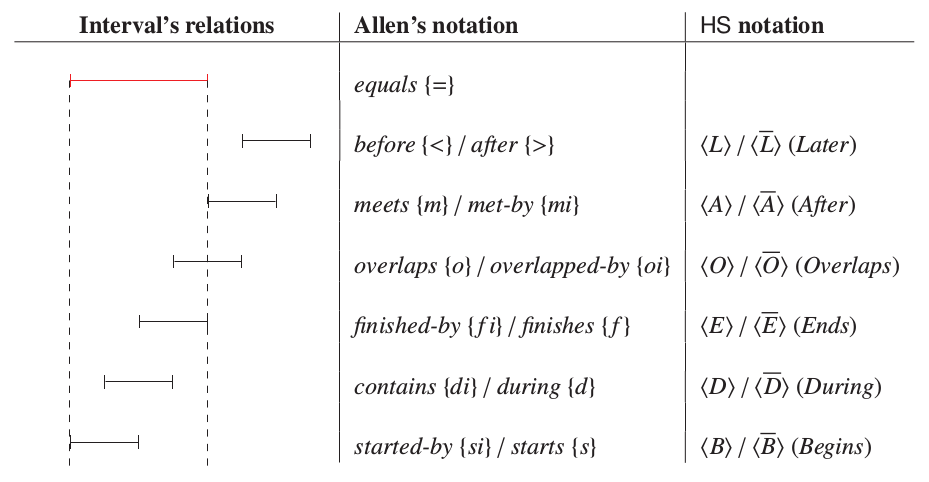
\includegraphics[height=2.5in]{itl.png}}
  \caption{Operators in the Interval Temporal Logic (taken from \cite{della2013interval})}
\end{figure}

\subsection{Propp Example with Punch and Judy}

In this example, we combine Halpern and Shoham's temporal operators with the possibility ($\Diamond$) and necessity ($\Box$) operators of modal logic. We follow the convention of writing possibility operators inside angle brackets: $\langle \, \rangle$ and necessity operators within square brackets: $[ \, ]$.

This example shows the ``sausages'' scene described in section \ref{sec:pjexample}, consisting of a set of situations $S$, containing Propp story functions $P$. The interval temporal logic operators used in this example are the set $T$.

\begin{align}
    S &= \{S_0, S_1, S_2, S_{3a}, S_{3a_1}, S_4, S_{3b}, S_{3b_1}, S_4, S_5\}\\
    P &= \{\mathtt{interdiction(A, B, C), absentation(A), struggle(A, B),}\nonumber\\
  &\qquad\qquad\mathtt{victory(A), villainy(A, B), violation(A, B), return(A)}\}\\
    T &= \{A, B, E\}
\end{align}

We use hybrid logic to identify nodes using the \emph{nominal} operator, shown as $\{\,\}$. 

\begin{align}
  &S_{0} \land \mathit{interdiction(Joey, Punch, Sausages)} \land\nonumber\\
  &\qquad\qquad\qquad\qquad\qquad\langle B \rangle \{S_{1}\} \land \langle E \rangle \{S_{4}\} \land \langle A \rangle \{S_{5}\}\\
  &[\{S_{1}\}] \mathit{absentation(Joey)} \land \langle A \rangle \{S_{2}\}\\
  &[\{S_{2}\}] \mathit{struggle(Punch, Crocodile)} \land \langle E \rangle (\{S_{3a}\} \lor \{S_{3b}\})\\
  &[\{S_{3a}\}] \mathit{victory(Crocodile)} \land \langle A \rangle \{S_{3a_1}\}\\
  &[\{S_{3a_1}\}] \mathit{villainy(Crocodile, Sausages)} \land \langle E \rangle \{S_{4}\}\\
  &[\{S_{3b}\}] \mathit{victory(Punch)} \land \langle A \rangle \{S_{3b_1}\}\\
  &[\{S_{3b_1}\}] \mathit{villainy(Punch, Sausages)} \land \langle E \rangle \{S_{4}\}\\
  &[\{S_{4}\}] \mathit{violation(Punch, Sausages)}\\
  &[\{S_{5}\}] \mathit{return(Joey)}
\end{align}



\section{Describing Punch and Judy with Kripke Structures}\label{sec:kripke}
We use Kripke structures \cite{kripke1963semantical} as a method of interpreting the combination of modal logic with Interval Temporal Logic. A Kripke structure is a graph, the nodes of which represent a possible world consisting of a set of assertions, and the edges of which are the accessibility relations between worlds.

\subsection{LoTREC}
LoTREC \cite{del2001lotrec} is a generic tableau prover for modal and description logics.

\subsection{The Sausages Scene in LoTREC}

\begin{figure}[!t]\label{fig:kripke}
  \centering
    \centerline{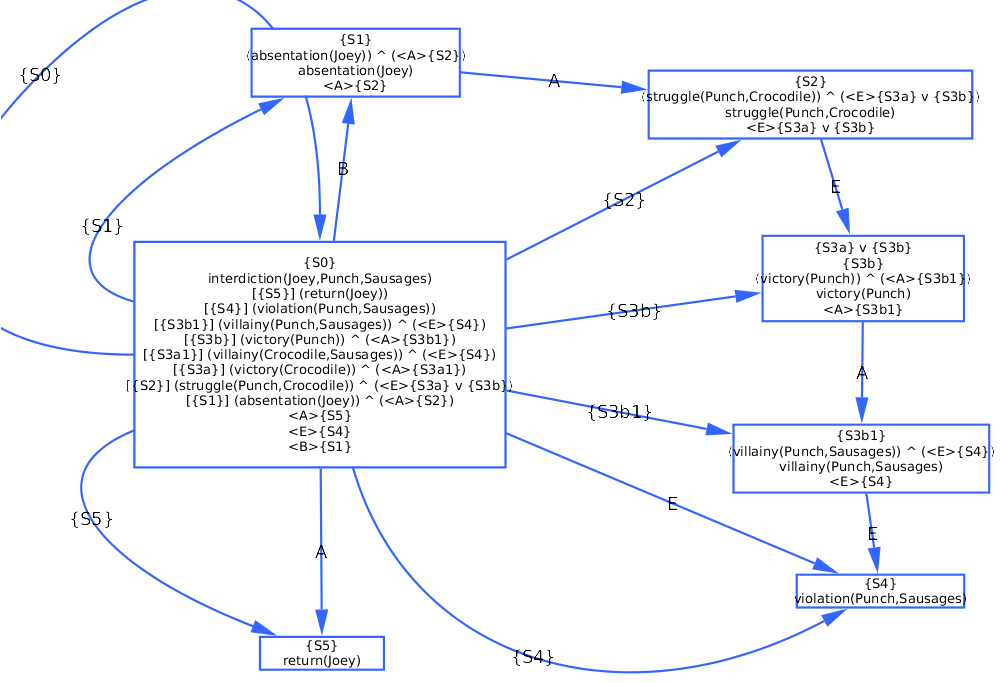
\includegraphics[height=3in]{kripke.png}}
  \caption{One premodel from the sausages scene in LoTREC}
\end{figure}

Figure \ref{fig:kripke} shows the premodel for the case where Punch wins the fight with the crocodile. One other premodel exists in this scenario, in which the crocodile is instead the victor.

\mnote{(Describe LoTREC, and how the sausages scene could be described in it)}

\section{Conclusions and Future Work}
\mnote{(Future work would be to use this system to regulate the actions of agents, hint at using in real-world applications like training systems)}
\jnote{This is a case study to try out this approach, with a view to applying in real-world situations}

\bibliography{icids}

\end{document}

